\chapter*{Ausarbeitung}

\section*{Aufgabe 1 Somigliana-Pizzetti-Normalpotential}

In der ersten Aufgabe dieser Übung soll aus der geozentrischen Gravitationskonstante $GM$, den Halbachsen $a$, $b$ des Referenzellipsoides und aus der Rotationsgeschwindigkeit der Erde $\omega$ der konstante Potentialwert $U_0$ des Somigliana-Pizzetti-Referenzpotentials auf dem Referenzellipsoid bestimmt werden. \\

Die exakte Darstellung des Normalpotentials in ellipsoidischen Koordinaten sieht wie folgt aus:

\begin{align}
U^{Ell}(\lambda,\beta,u) = \left(U_0 - \dfrac{\omega^2 a^2}{3}\right) \dfrac{Q_{0,0}^{*}\left(\dfrac{u}{E}\right)}{{Q_{0,0}^{*}\left(\dfrac{b}{E}\right)}} + \dfrac{\omega^2 a^2 Q_{2,0}^{*}\left(\dfrac{u}{E}\right)}{3 Q_{2,0}^{*}\left(\dfrac{b}{E}\right)} P_{2,0}(\sin \beta)
\end{align}

mit $E = \sqrt{a^2 - b^2}$, und 

\begin{align*}
Q_{0,0}^{*}\left(\dfrac{u}{E}\right) &= \arctan \left(\dfrac{E}{u}\right) \\
Q_{2,0}^{*}\left(\dfrac{b}{E}\right) &= \dfrac{1}{2} \left[\left(3 \left(\dfrac{b}{E}\right)^2+1\right) \text{arccot} \left(\dfrac{b}{E}\right)-3 \left(\dfrac{b}{E}\right)\right]
\end{align*}

Die Darstellung des Normalpotentials in sphärischen Koordinaten lautet: 

\begin{align}
U^{Sph}(\lambda,\varphi,r)= \dfrac{GM}{r} \left[1-\sum_{n=1}^{L} \left(\dfrac{a}{r}\right)^{2n} J_{2n} P_{2n} (\sin \varphi)\right] + \dfrac{\omega^2}{2} r^2 \cos^2 \varphi
\end{align}

mit 

\begin{align*}
J_2 &= \dfrac{e^2}{3} \left(1-\dfrac{2}{15} \dfrac{e'\hat{m}}{q_0}\right) \\
J_{2n} &= (-1)^{n+1} \dfrac{3e^{2n}}{(2n+1)(2n+3)} \left(1-n+5n \dfrac{J_2}{e^2}\right) ~~~~~ n > 1 
\end{align*}

Des Weiteren gilt:

\begin{gather*}
e = \dfrac{E}{a}, ~~~~~ e'= \dfrac{E}{b} \\
\hat{m} = \dfrac{\omega^2 a^2 b }{GM}, ~~~~~ q_0 = Q_{2,0}^{*} \left(\dfrac{b}{E}\right)
\end{gather*}

Im ersten Schritt gilt es beide Darstellungen des Potentials mit dem Radius $r$ zu multiplizieren und folglich die Grenzwerte 	\dq im Unendlichen\dq zu betrachten. Somit gilt: 

\begin{align*}
\lim_{r \rightarrow \infty} r \cdot U^{Ell}(\lambda,\beta,u) = \lim_{r \rightarrow \infty} r \cdot \left(\left(U_0 - \dfrac{\omega^2 a^2}{3}\right) \dfrac{Q_{0,0}^{*}\left(\dfrac{u}{E}\right)}{{Q_{0,0}^{*}\left(\dfrac{b}{E}\right)}} + \dfrac{\omega^2 a^2 Q_{2,0}^{*}\left(\dfrac{u}{E}\right)}{3 Q_{2,0}^{*}\left(\dfrac{b}{E}\right)} P_{2,0}(\sin \beta)\right) = GM
\end{align*}

beziehungsweise

\begin{align*}
\lim_{r \rightarrow \infty} r \cdot U^{Sph}(\lambda,\varphi,r) = \lim_{r \rightarrow \infty} r \cdot \left(\dfrac{GM}{r} \left[1-\sum_{n=1}^{L} \left(\dfrac{a}{r}\right)^{2n} J_{2n} P_{2n} (\sin \varphi)\right] + \dfrac{\omega^2}{2} r^2 \cos^2 \varphi\right) = GM
\end{align*}

\section*{Aufgabe 2}

\begin{enumerate}
\item In dieser Teilaufgabe wird für das Somigliana-Pizzetti-Normalpotential die Konvergenz der Reihenentwicklungen für die Entwicklungsgrade $L=2,4,6,8$ diskutiert. Anschließend werden die Ergebnisse visualisiert.

\begin{figure}[H]
\centering
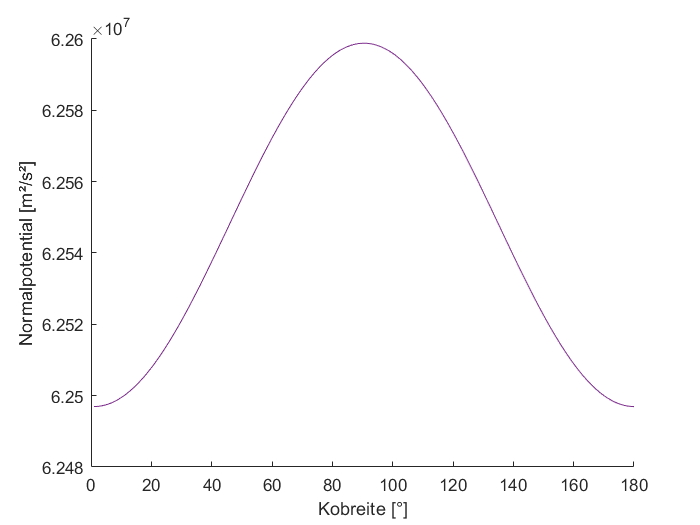
\includegraphics[scale=0.6]{ergeb.png}
\caption{Visualisierung der Ergebnisse}
\label{ergeb}
\end{figure}

In Abbildung \ref{ergeb} sieht man die Ergebnisse der Konvergenz der Reihenentwicklungen für die Entwicklungsgrade $L=2,4,6,8$ in Abhängigkeit von der Cobreite $\varphi$. Der Abbildung ist zu entnehmen, dass tatsächlich die Ergebnisse aller vier Entwicklungsgrade sich nahezu überlagern. Insofern sind keine klaren vier Kurven zu erkennen. Numerische Abweichungen treten zwar auf, sind aber dennoch sehr gering. Daraus kann man also schließen, dass die Variation des Entwicklungsgrades keinen besonders großen Einfluss auf die Ergebnisse hat. Zudem lässt sich erkennen, dass die Graphen einen Abschnitt einer harmonischen Funktion darstellen. Hierbei ist bei $90^{\circ}$, also am Äquator, das Maximum.   

\item Im zweiten Teil dieser Aufgabe wird das Somigliana-Pizzetti-Normalpotential zum Grad $L_{max}=8$ und das volle Schwerepotential (Modell EGM96 mit dem Entwicklungsgrad $L_{max} = 36$) verglichen. Hierbei werden die Entwicklungen auf einer Kugel um das Geozentrum mit Radius 6371 km ausgewertet. In farbcodierten Erdkarten werden anschließend die Potentiale, sowie deren Differenzen dargestellt. Zuletzt sollen auch die entsprechenden Werte entlang des Meridians durch Greenwich visualisiert werden. 

\begin{figure}[H]
	\centering
	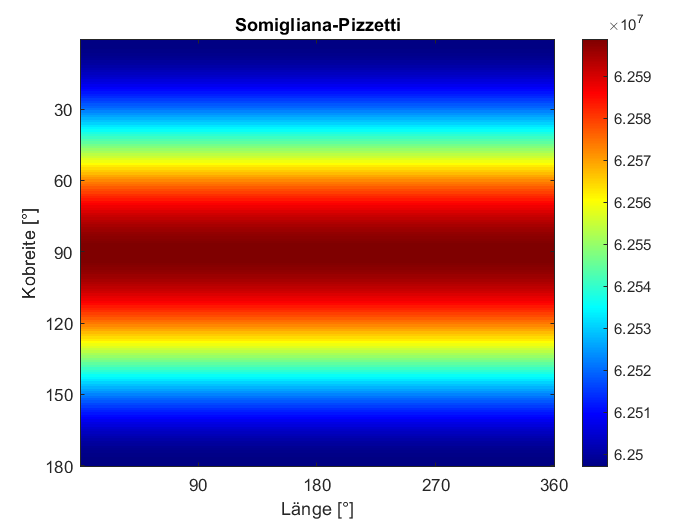
\includegraphics[scale=0.6]{SP.png}
	\caption{Somigliana-Pizzetti}
	\label{sp}
\end{figure}

Abbildung \ref{sp} stellt das Somigliana-Pizzetti-Normalpotential zum Grad $L_{max}=8$ dar.

\begin{figure}[H]
	\centering
	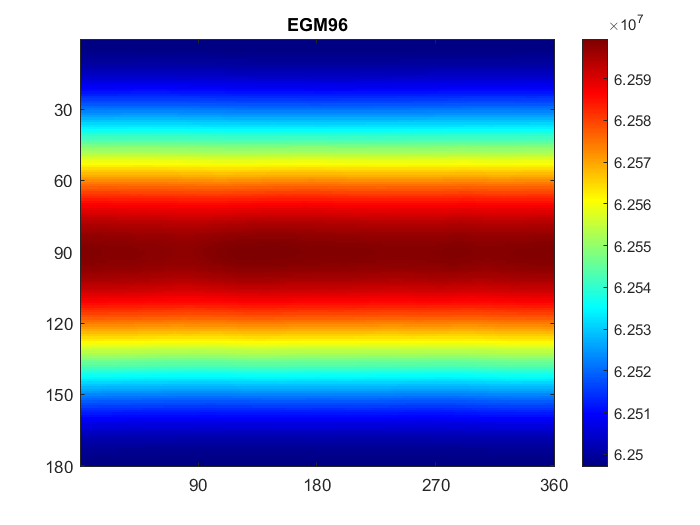
\includegraphics[scale=0.6]{egm96.png}
	\caption{EGM96}
	\label{egm96}
\end{figure}

Abbildung \ref{egm96} stellt das volle Schwerepotential zum Grad $L_{max}=36$ dar.

\begin{figure}[H]
	\centering
	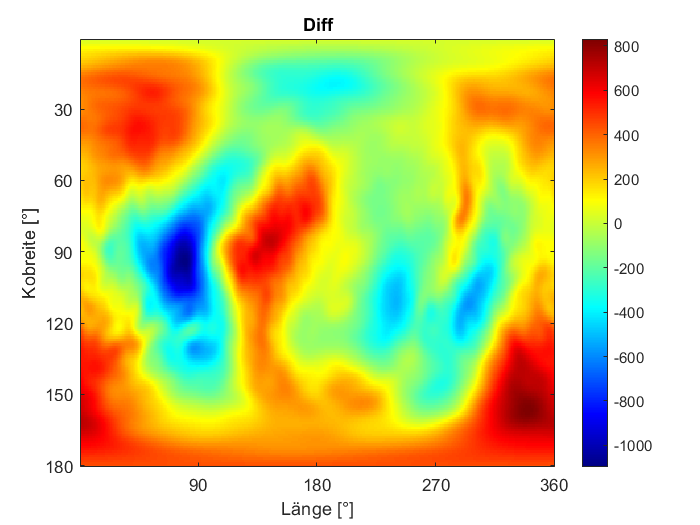
\includegraphics[scale=0.6]{diff.png}
	\caption{Differenz der beiden Potentiale}
	\label{diff}
\end{figure}

In Abbildung \ref{diff} sieht man die Differenz der beiden Potentiale dargestellt als farbcodierte Erdkarten. 

 
\end{enumerate}
